%----------------------------------------------------------------------------------------
%	PACKAGES AND OTHER DOCUMENT CONFIGURATIONS
%----------------------------------------------------------------------------------------

\documentclass[landscape,a0paper,fontscale=0.285]{baposter} % Adjust the font scale/size here

\usepackage{graphicx} % Required for including images
\graphicspath{{figures/}} % Directory in which figures are stored

\usepackage{amsmath} % For typesetting math
\usepackage{amssymb} % Adds new symbols to be used in math mode

\usepackage{booktabs} % Top and bottom rules for tables
\usepackage{enumitem} % Used to reduce itemize/enumerate spacing
\usepackage{palatino} % Use the Palatino font
\usepackage[font=small,labelfont=bf]{caption} % Required for specifying captions to tables and figures

\usepackage{multicol} % Required for multiple columns
\setlength{\columnsep}{1.5em} % Slightly increase the space between columns
\setlength{\columnseprule}{0mm} % No horizontal rule between columns

\usepackage{tikz} % Required for flow chart
\usetikzlibrary{shapes,arrows} % Tikz libraries required for the flow chart in the template

\newcommand{\compresslist}{ % Define a command to reduce spacing within itemize/enumerate environments, this is used right after \begin{itemize} or \begin{enumerate}
\setlength{\itemsep}{1pt}
\setlength{\parskip}{0pt}
\setlength{\parsep}{0pt}
}

\definecolor{lightblue}{rgb}{0.145,0.6666,1} % Defines the color used for content box headers

\begin{document}

\begin{poster}
{
headerborder=closed, % Adds a border around the header of content boxes
colspacing=1em, % Column spacing
bgColorOne=white, % Background color for the gradient on the left side of the poster
bgColorTwo=white, % Background color for the gradient on the right side of the poster
borderColor=lightblue, % Border color
headerColorOne=black, % Background color for the header in the content boxes (left side)
headerColorTwo=lightblue, % Background color for the header in the content boxes (right side)
headerFontColor=white, % Text color for the header text in the content boxes
boxColorOne=white, % Background color of the content boxes
textborder=roundedleft, % Format of the border around content boxes, can be: none, bars, coils, triangles, rectangle, rounded, roundedsmall, roundedright or faded
eyecatcher=true, % Set to false for ignoring the left logo in the title and move the title left
headerheight=0.1\textheight, % Height of the header
headershape=roundedright, % Specify the rounded corner in the content box headers, can be: rectangle, small-rounded, roundedright, roundedleft or rounded
headerfont=\Large\bf\textsc, % Large, bold and sans serif font in the headers of content boxes
%textfont={\setlength{\parindent}{1.5em}}, % Uncomment for paragraph indentation
linewidth=2pt % Width of the border lines around content boxes
}
%----------------------------------------------------------------------------------------
%	TITLE SECTION
%----------------------------------------------------------------------------------------
%
{
\includegraphics[height=5em]{logo.png}} % First university/lab logo on the left
{\bf\textsc{Albo Hessab Mini Webpage}\vspace{0.5em}} % Poster title
{\textsc{ Miliyon T.\\ \hspace{12pt} Addis Ababa University, Mathematics Department}} % Author names and institution
{
\includegraphics[height=5em]{logo.png}} % Second university/lab logo on the right

%----------------------------------------------------------------------------------------
%	OBJECTIVES
%----------------------------------------------------------------------------------------

\headerbox{Objectives}{name=objectives,column=0,row=0}{

The main objective of this site is to help undergraduate Mathematics Major students here in Addis Ababa University.
By providing resources that are very useful for the learning process. Such as

\begin{enumerate}\compresslist
\item Course outlines
\item Lecture notes
\item Texts(Available)
\item Books
\item etc.
\end{enumerate}

\vspace{0.3em} % When there are two boxes, some whitespace may need to be added if the one on the right has more content
}

%----------------------------------------------------------------------------------------
%	INTRODUCTION
%----------------------------------------------------------------------------------------

\headerbox{Introduction}{name=introduction,column=1,row=0,bottomaligned=objectives}{

"If you have to begin, begin from the ground. If you have to start, start from your own."
\begin{flushright}
-Anonymous.
\end{flushright}
Freshman year was quite tough for me. So I asked myself can  I make it much simpler for my young brothers? I started thinking about designing a web-page. Immediately I start to collect resources from my teachers[You deserve more than Thank you].
I did everything during the semester break. That is why it took me so long. Anyways here it is finally.
}

%----------------------------------------------------------------------------------------
%	RESULTS 1
%----------------------------------------------------------------------------------------

\headerbox{Overview}{name=results,column=2,span=2,row=0}{

\begin{multicols}{2}
\vspace{1em}
\begin{center}
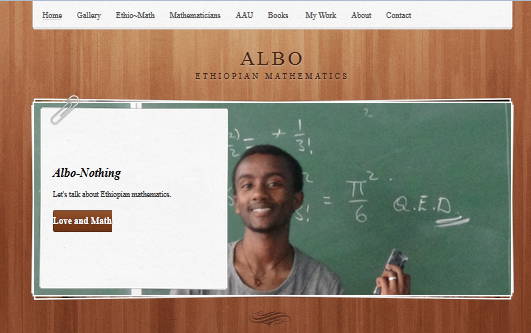
\includegraphics[width=1.9\linewidth]{placeholder}
\captionof{figure}{Homepage}
\end{center}


\end{multicols}

%------------------------------------------------

\begin{multicols}{2}
\vspace{1em}

\begin{center}
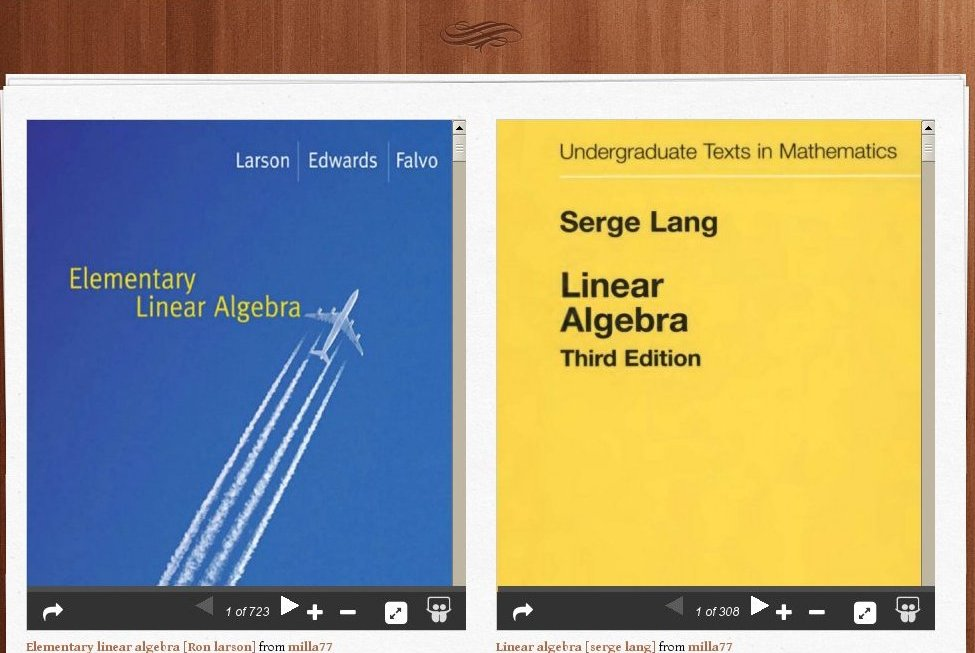
\includegraphics[width=0.8\linewidth]{pbook}
\captionof{figure}{Books}
\end{center}

\begin{center}
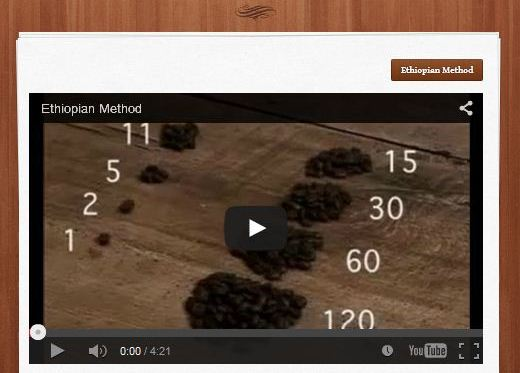
\includegraphics[width=0.7\linewidth]{pplace}
\captionof{figure}{Ethio-Math}
\end{center}

\end{multicols}
}

%----------------------------------------------------------------------------------------
%	REFERENCES
%----------------------------------------------------------------------------------------

\headerbox{Acknowledgement}{name=references,column=0,above=bottom}{

\renewcommand{\section}[2]{\vskip 0.05em} % Get rid of the default "References" section title
\nocite{*} % Insert publications even if they are not cited in the poster
\small{ % Reduce the font size in this block
\bibliographystyle{unsrt}
\bibliography{sample} % Use sample.bib as the bibliography file
}}

%----------------------------------------------------------------------------------------
%	FUTURE RESEARCH
%----------------------------------------------------------------------------------------

\headerbox{Future Plan}{name=futureresearch,column=1,span=2,aligned=references,above=bottom}{ % This block is as tall as the references block

\begin{multicols}{2}
-To provide more resources.

-To make the page attractive and easily accessible.


-To upgrade the domain.
\end{multicols}
}

%----------------------------------------------------------------------------------------
%	CONTACT INFORMATION
%----------------------------------------------------------------------------------------

\headerbox{Contact Information}{name=contact,column=3,aligned=references,above=bottom}{ % This block is as tall as the references block

\begin{description}\compresslist
\item[Web:] www.albohessab.weebly.com
\item[Email:] miliyon@ymail.com
\item[Phone:] +251 (000) 911 90 1234
\end{description}
}

%----------------------------------------------------------------------------------------
%	CONCLUSION
%----------------------------------------------------------------------------------------

\headerbox{Comment}{name=conclusion,column=2,span=2,row=0,below=results,above=references}{

\begin{multicols}{2}


\begin{itemize}\compresslist
\item I appreciate any comment from anyone.
\end{itemize}

\end{multicols}
}

%----------------------------------------------------------------------------------------
%	MATERIALS AND METHODS
%----------------------------------------------------------------------------------------

\headerbox{Ethiopian Numerals}{name=method,column=0,below=objectives,bottomaligned=conclusion}{ % This block's bottom aligns with the bottom of the conclusion block

Do we really know our own numeral system?

\begin{center}
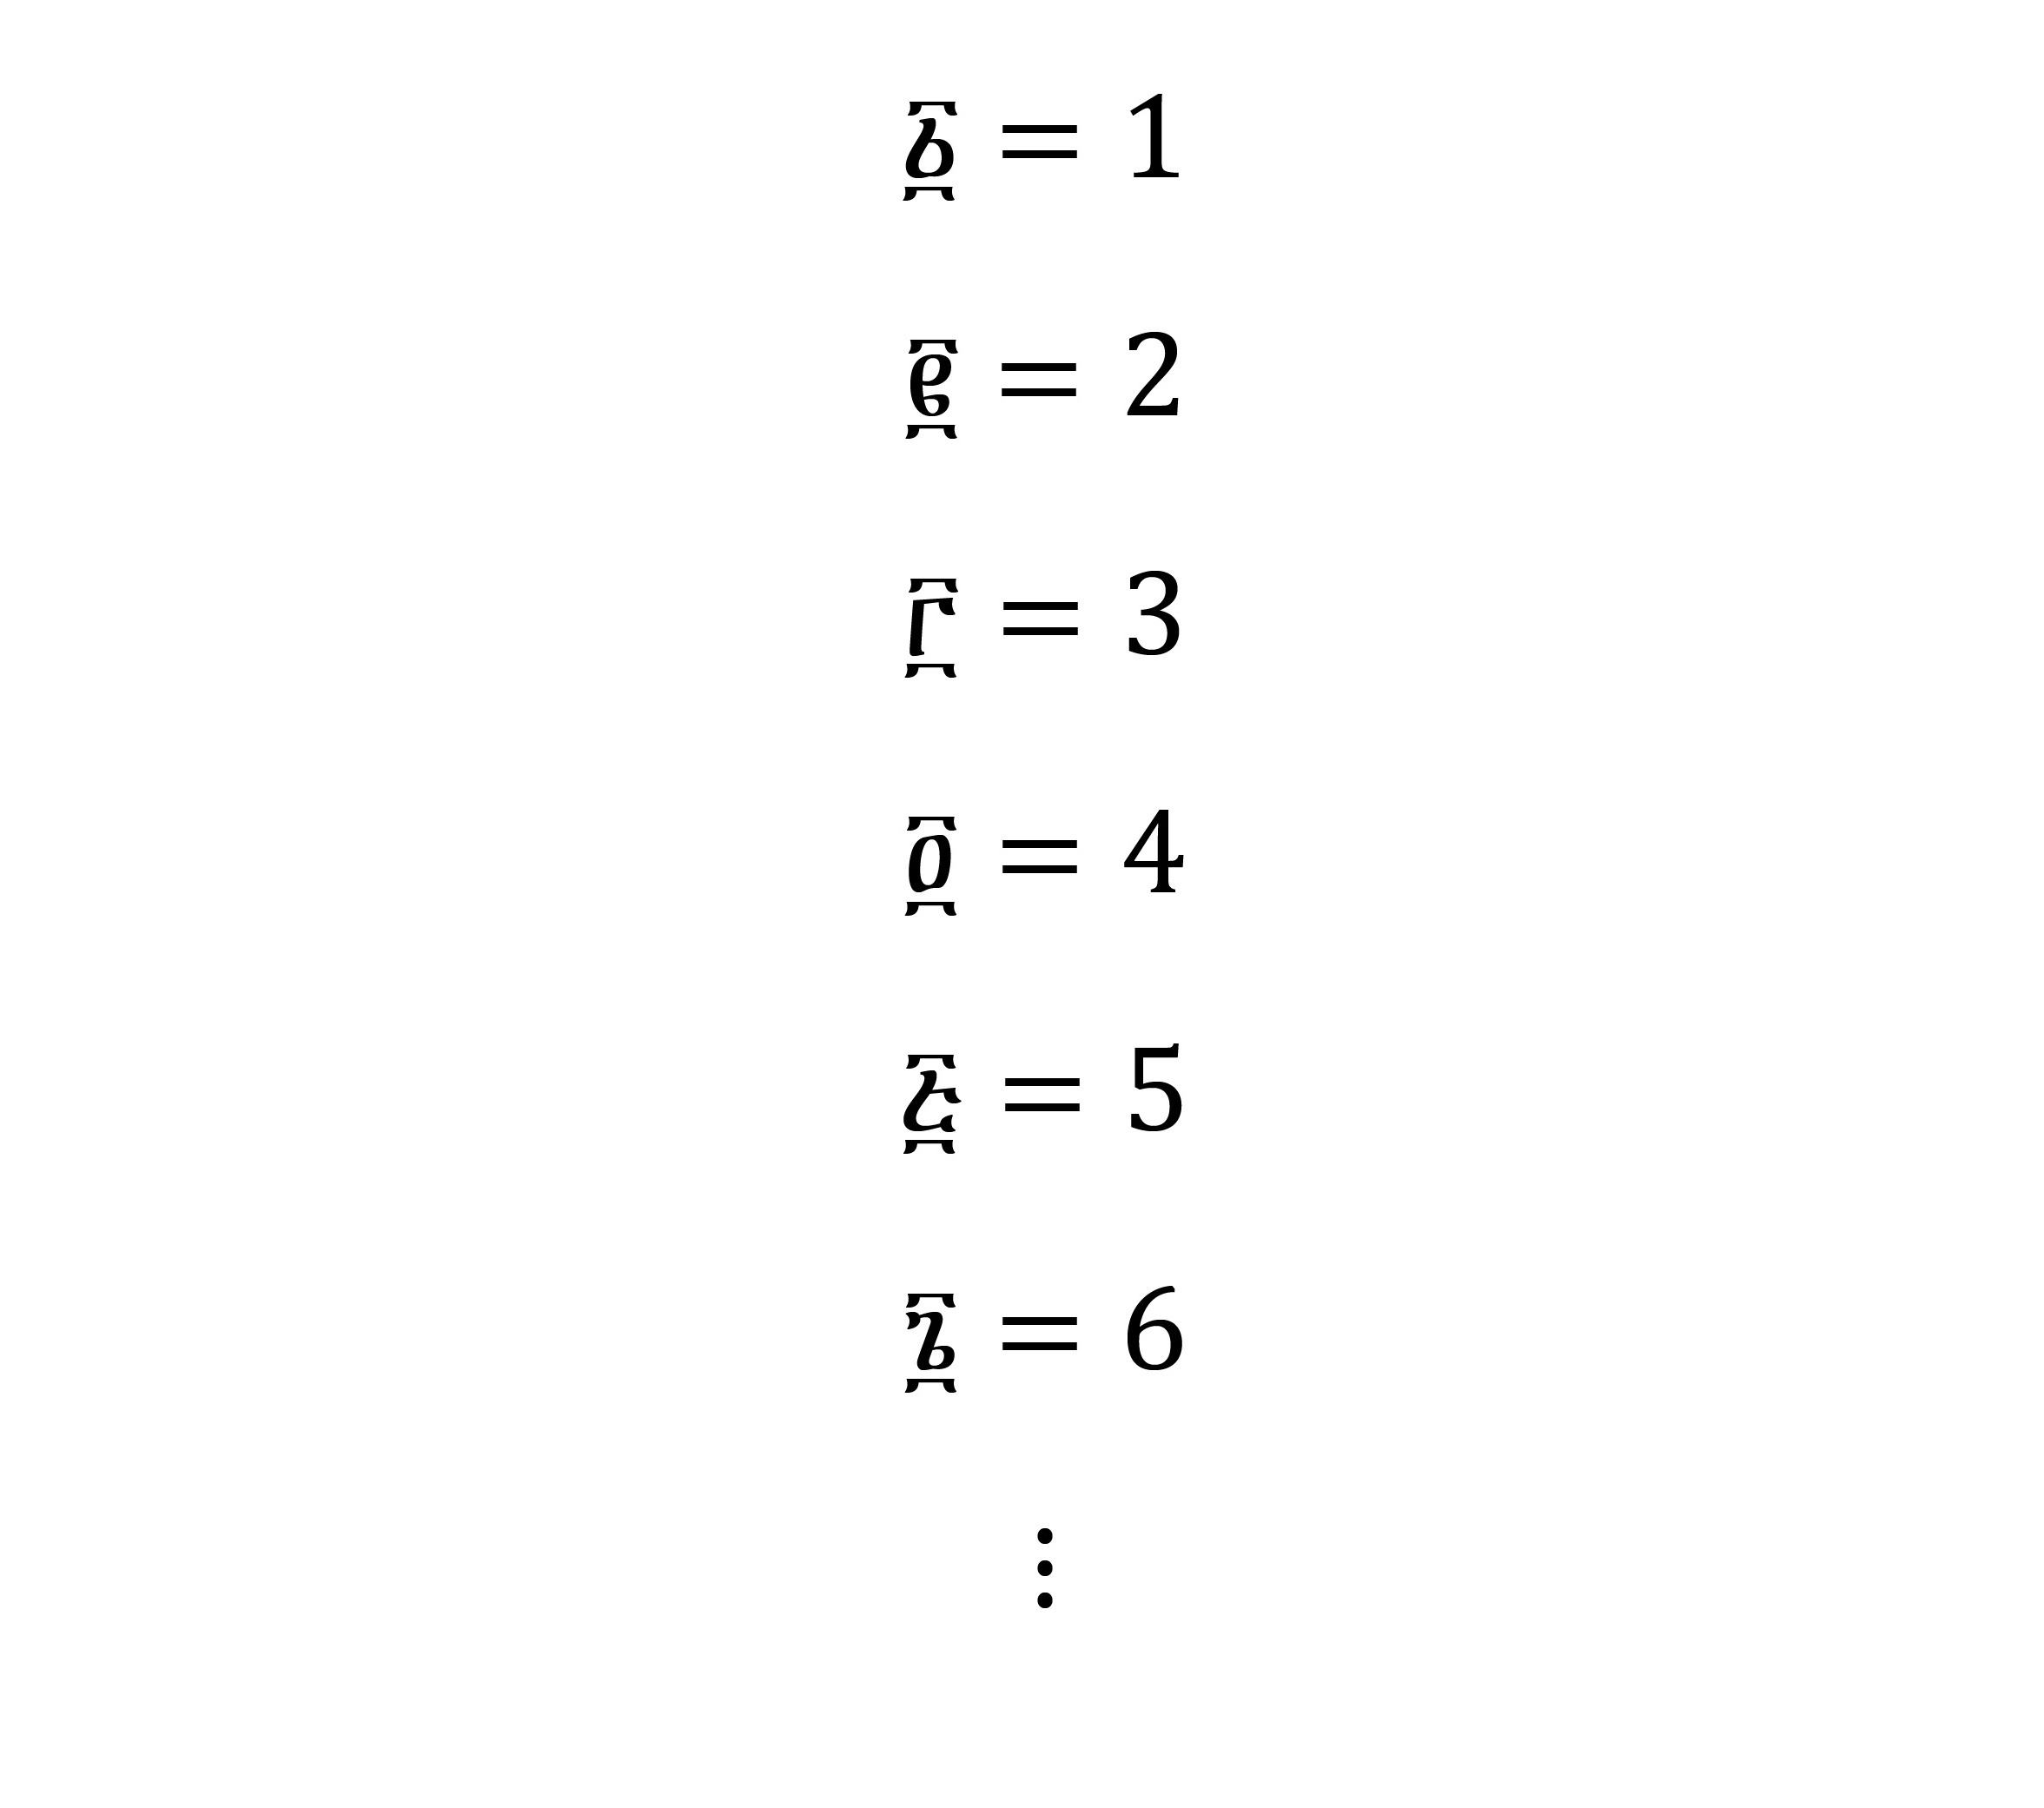
\includegraphics[width=0.8\linewidth]{place}
\end{center}

There are lots of ambiguity about Ethiopian Numerals. For example

Do ancient Ethiopians know the number zero?
There are more to be asked. I hope together we will find the answer to all this questions.

Let's Collaborate and see the difference.
}

%----------------------------------------------------------------------------------------
%	RESULTS 2
%----------------------------------------------------------------------------------------

\headerbox{Blog}{name=results2,column=1,below=objectives,bottomaligned=conclusion}{ % This block's bottom aligns with the bottom of the conclusion block

At the right corner of the web-page there is a blog which is created to provide news, and announcement like Seminar and special events.
\begin{center}
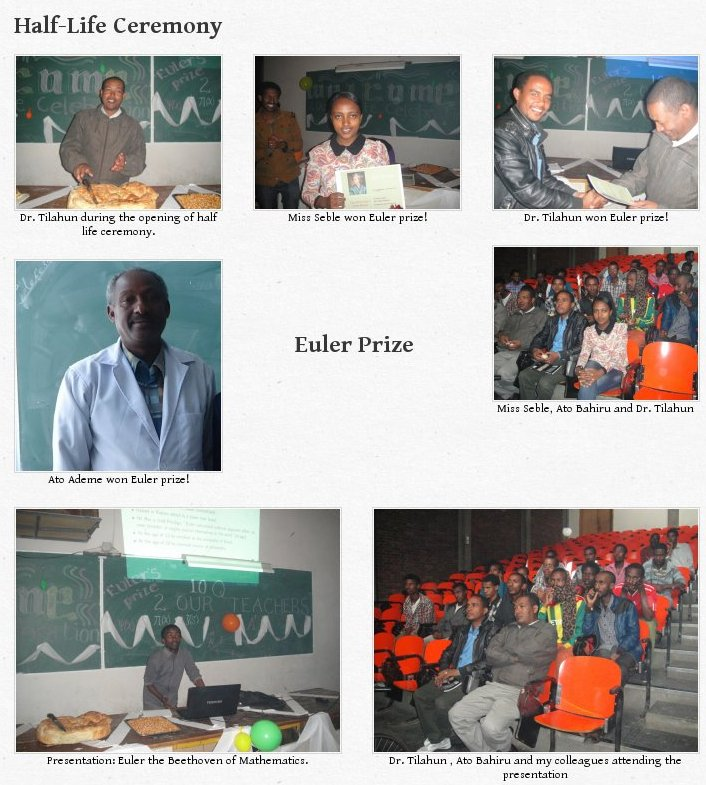
\includegraphics[width=0.8\linewidth]{palace}
\end{center}

I need you to contribute for this blog. If there is anything that you think important, please forward it.
Let's share what we know!
}

%----------------------------------------------------------------------------------------

\end{poster}

\end{document}
